\newpage
\begin{center}
    \textbf{BAB II}\\
    \textbf{LANDASAN TEORI DAN KERANGKA BERPIKIR}
    \addcontentsline{toc}{chapter}{BAB II. LANDASAN TEORI DAN KERANGKA BERPIKIR}
\end{center}

\textbf{A. Landasan Teori}
\addcontentsline{toc}{section}{A. Landasan Teori}
\begin{enumerate}
    \item Pendidikan Matematika\\
    \hspace*{1cm}Pentingnya pendidikan matematika didasarkan pada fakta bahwa matematika merupakan aktivitas dasar manusia, sebagaimana halnya musik, seni lukis, sastra, atau pembuatan sepatu berkualitas \citep{hilton1984}. Matematika murni membentuk lingkungan tempat aktivitas sehari-hari manusia berlangsung \citep{yig2022}. Menurut Schoenfeld (2000), pendidikan matematika memiliki dua tujuan utama: tujuan murni untuk memahami cara berpikir matematis dan pengajarannya, serta tujuan terapan untuk meningkatkan kualitas pengajaran matematika. Matematika merupakan elemen mendasar dalam sains, teknologi, dan pemahaman lingkungan. Agar pendidikan matematika berhasil, bidang matematika murni dan terapan harus disajikan secara seimbang \citep{hilton1984}. Karena terdapat hubungan timbal balik antara keduanya, pemahaman mendalam mengenai cara berpikir, belajar, dan mengajar matematika sangat penting untuk mengembangkan praktik pembelajaran berkelanjutan \citep{schoenfeld2000}.\\
    \hspace*{1cm}Pendidikan matematika merupakan disiplin ilmu yang menggunakan berbagai konsep dan topik secara intensif \citep{turkdogan2015}. Penggunaan konsep-konsep dan hubungan antar konsep merupakan komponen penting dalam bidang ini. Dengan pemahaman yang tepat, pendidikan matematika memberikan perspektif baru bagi peneliti untuk menelaah topik lebih mendalam, mengajukan pertanyaan baru, dan menemukan alternatif-alternatif inovatif \citep{ernest2016}. Schoenfeld (2000) mengemukakan beberapa pertanyaan utama dalam pendidikan matematika:
    \begin{enumerate}
        \item Perspektif teoritis untuk memahami pemikiran, pembelajaran, dan pengajaran;
        \item Berbagai aspek kognisi (misalnya pemikiran matematis, pemahaman siswa, dan kesalahpahaman);
        \item Bukti keberhasilan (situasi di mana siswa dapat belajar memecahkan masalah, induksi, interaksi kelompok, dan penerapan berbagai jenis pengajaran);
        \item Konsekuensi dari berbagai bentuk pengajaran (baik yang bersifat positif maupun negatif).
    \end{enumerate}
    \hspace*{1cm}Dari uraian tersebut dapat disimpulkan bahwa pendidikan matematika memiliki peran penting dalam membentuk pola pikir, meningkatkan kualitas pembelajaran serta mendukung perkembangan ilmu pengetahuan dan teknologi. Keberhasilan pendidikan matematika bergantung pada keseimbangan antara pemahaman konsep teoritis dan penerapannya dalam konteks nyata. Dengan pendekatan dan pemahaman yang tepat, pendidikan matematika dapat berkontribusi dalam menciptakan pembelajaran bermakna dan berkelanjutan.

    \item \textit{Augmented Reality}\\
    \hspace*{1cm}\textit{Augmented Reality} (AR) memungkinkan penempatan objek virtual yang dihasilkan komputer di atas objek fisik secara \textit{real-time} \citep{ozdemir2018}. Penggabungan antara dunia nyata dan dunia maya membuat batas di antara keduanya sangat tipis. AR memiliki tiga karakteristik utama: (1) menggabungkan dunia nyata dan virtual; (2) interaktif secara \textit{real-time}; dan (3) mampu menyajikan tampilan tiga dimensi \citep{azuma1997}. Teknologi ini dapat memuat video, suara, gambar, teks, dan model 3D \citep{tekedere2016}. Pengguna dapat berinteraksi dengan objek virtual dalam lingkungan sekitarnya dan memperoleh pengalaman interaktif dengan komputer \citep{cai2014}. Dalam pembelajaran, AR memungkinkan siswa menjelajahi dunia secara interaktif dan kolaboratif \citep{antonioli2014}. Multimedia interaktif berbasis AR menyediakan fasilitas bagi pengguna untuk berinteraksi dengan objek 3D, membantu siswa memahami konsep dengan lebih mudah \citep{martin2010}.\\
    \hspace*{1cm}Penggunaan teknologi AR berkontribusi terhadap perkembangan siswa dalam aspek afektif dan kognitif, menjadikan pembelajaran lebih efisien dan menarik \citep{tomi2013}. Pembelajaran berbasis AR juga efektif dalam kegiatan tatap muka \citep{lin2013}. Selain itu, AR memberikan kontribusi positif dalam proses belajar dengan meningkatkan pemahaman, persepsi konsep, dan membantu siswa berpikir terstruktur, terutama pada mata pelajaran sains dan matematika \citep{bujak2013}.\\
    \hspace*{1cm}Kesimpulannya, teknologi AR memiliki potensi besar dalam mengembangkan kemampuan spasial siswa. Dengan menggabungkan dunia nyata dan virtual secara interaktif dan real-time, AR menyajikan pengalaman belajar imersif melalui tampilan 3D. Teknologi ini tidak hanya memperkaya aspek kognitif dan afektif siswa, tetapi juga memudahkan pemahaman konsep-konsep abstrak melalui visualisasi konkret. Oleh karena itu, integrasi AR dalam pembelajaran, khususnya sains dan matematika, merupakan alternatif inovatif yang meningkatkan efektivitas, keterlibatan, dan pemahaman siswa.

    \item Kemampuan Spasial dan Teknologi\\
    \hspace*{1cm}Berbagai istilah digunakan dalam literatur untuk mendefinisikan kemampuan spasial, antara lain: pemikiran spasial \citep{yakimanskaya1991}, pengertian spasial \citep{nctm1989}, keterampilan spasial \citep{tartre1990}, dan penalaran spasial \citep{battista2007} \citep{ozcakir2021augmented}. Secara umum, kemampuan spasial mengacu pada kemampuan untuk memutar, mengubah, membayangkan suatu objek serta memanipulasi sifat-sifatnya secara mental \citep{ozcakir2021augmented}. Dengan kata lain, kemampuan spasial adalah keterampilan dalam membayangkan bentuk-bentuk geometri dan perubahan bentuk tersebut ketika diputar atau dimanipulasi dalam pikiran.\\
    \hspace*{1cm}Beberapa peneliti mengklasifikasikan kemampuan spasial berbeda-beda. \citet{battista1994} membaginya menjadi dua komponen: orientasi spasial dan visualisasi spasial. \citet{pellegrino1982} membedakan antara hubungan spasial dan visualisasi spasial. \citet{linn1985} membagi menjadi tiga elemen: perputaran mental, persepsi spasial, dan visualisasi spasial. Meskipun perbedaan ini ada, semua komponen tersebut dapat dipahami secara logis dan relevan dengan kemampuan berpikir spasial manusia \citep{ozcakir2021augmented}. \citet{maier1996} mengusulkan lima elemen kemampuan spasial: perputaran mental, persepsi spasial, visualisasi spasial, hubungan spasial, dan orientasi spasial, menekankan bahwa kemajuan teknologi menuntut pelatihan menyeluruh terhadap kelima elemen ini untuk pengembangan keterampilan spasial yang mendalam.\\
    \hspace*{1cm}Secara ringkas, kemampuan spasial merupakan aspek kognitif penting yang melibatkan visualisasi, manipulasi, dan rotasi objek secara mental. Pelatihan terhadap komponen-komponen kemampuan spasial menjadi semakin penting seiring perkembangan teknologi, khususnya dalam pendidikan untuk meningkatkan efektivitas pemahaman konsep-konsep abstrak yang membutuhkan representasi visual.

    \item Bangun Ruang Sisi Datar\\
    \hspace*{1cm}Berdasarkan Permendikbud Nomor 37 Tahun 2018 tentang Kompetensi Inti dan Kompetensi Dasar, materi Matematika SMP Kelas VIII Semester Genap mencakup pembahasan tentang bangun ruang sisi datar. Penelitian ini difokuskan pada materi tersebut, dengan kompetensi dasar yang ditampilkan pada Tabel \ref{kikd} berikut:
    \begin{table}[H]
        \centering
        \caption{KI dan KD Materi Bangun Ruang Sisi Datar}
        \label{kikd}
        \begin{tabular}{|p{7cm}|p{7cm}|}
            \hline
            \textbf{Kompetensi Inti 3 (Pengetahuan)} & \textbf{Kompetensi Inti 4 (Keterampilan)} \\
            \hline
            Memahami dan menerapkan pengetahuan (faktual, konseptual, dan prosedural) berdasarkan rasa ingin tahunya tentang ilmu pengetahuan, teknologi, seni, budaya terkait fenomena dan kejadian tampak mata. &
            Mengolah, menyaji dan menalar dalam ranah konkret (menggunakan, mengurai, merangkai, memodifikasi, dan membuat) dan ranah abstrak (menulis, membaca, menghitung, menggambar, dan mengarang) sesuai dengan yang dipelajari di sekolah dan sumber lain yang sama dalam sudut pandang/teori. \\
            \hline
            \textbf{Kompetensi Dasar 3.9} & \textbf{Kompetensi Dasar 4.9}\\
            \hline
            Membedakan dan menentukan luas permukaan dan volume bangun ruang sisi datar (kubus, balok, prisma, limas). & Menyelesaikan masalah yang berkaitan dengan luas permukaan dan volume bangun ruang sisi datar (kubus, balok, prisma, dan limas), serta gabungannya.\\
            \hline
        \end{tabular}
    \end{table}
    \hspace*{1cm}Jenis bangun ruang sisi datar yang dibahas dalam materi SMP meliputi kubus, balok, prisma, dan limas. Pembahasan difokuskan pada volume dan luas permukaan bangun ruang tersebut.
    \begin{enumerate}
        \item Luas Permukaan\\
        \hspace*{1cm}Luas permukaan adalah jumlah luas seluruh sisi suatu bangun ruang. Sebagai contoh, pada kubus, luas permukaan merupakan jumlah luas dari keenam sisinya. Karena kubus memiliki enam sisi yang kongruen (sama besar), maka luas permukaan kubus dapat dihitung dengan mengalikan luas satu sisi dengan enam. Penjelasan lebih lanjut dapat dilihat pada Gambar \ref{kubusjaring}.
        \begin{figure}[H]
            \centering
            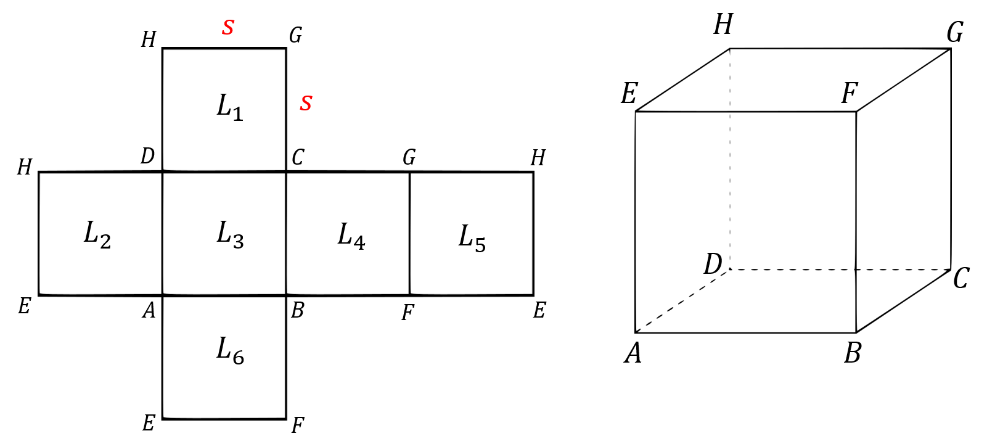
\includegraphics[width=0.6\textwidth]{images/kubusdanjaring.png}
            \caption{Kubus dan Jaring-jaringnya}
            \label{kubusjaring}
        \end{figure}
        \hspace*{1cm}Pada Gambar \ref{kubusjaring}, disajikan kubus dengan enam buah sisi sama besar.\\
        \( L_1 = L_2 = L_3 = L_4 = L_5 = L_6 \)

        Sehingga seluruh luas permukaan kubus adalah\\
        $ L = L_1 + L_2 + L_3 + L_4 + L_5 + L_6 $\\
        $ L = 6 \times L_1 $\\
        $ L = 6 \times s \times s = 6 \times s^2 .$\\
        Cara mencari luas permukaan balok sedikit berbeda dengan kubus karena ukuran sisi-sisinya tidak semuanya sama. Perbedaan ini ditunjukkan pada Gambar \ref{balokjaring}.
        \begin{figure}[H]
            \centering
            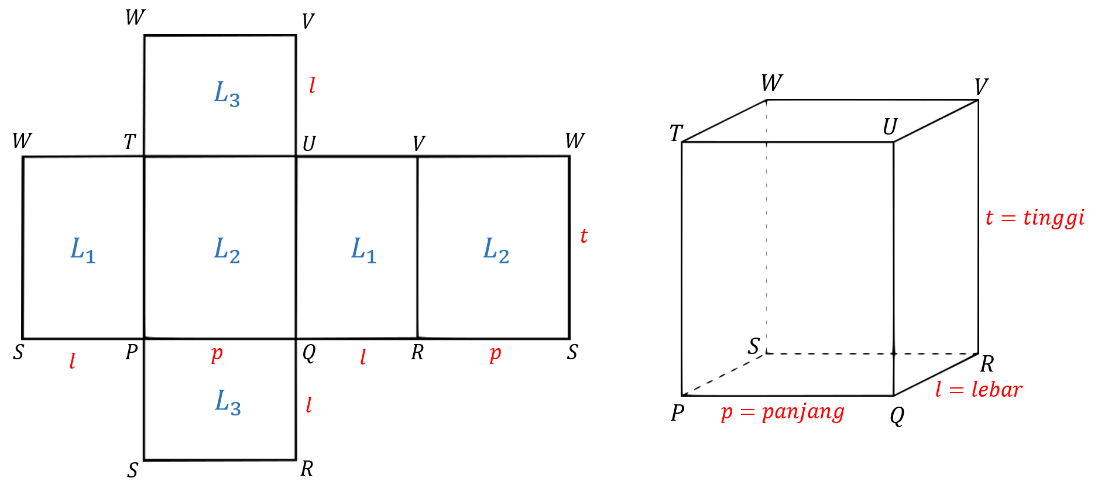
\includegraphics[width=0.6\textwidth]{images/balokdanjaring.png}
            \caption{Balok dan Jaring-jaringnya}
            \label{balokjaring}
        \end{figure}
        \hspace*{1cm}Pada bangun balok, sisi-sisi yang berhadapan memiliki ukuran yang sama. Misalnya, sisi depan sama dengan sisi belakang, sisi kiri sama dengan sisi kanan, serta sisi atas sama dengan sisi bawah. Pada Gambar 2, masing-masing sisi diberi label untuk mempermudah pemahaman. Luas permukaan balok dirumuskan sebagai berikut:\\
        $ L = 2 \times L_1 + 2 \times L_2 + 2 \times L_3 $\\
        $ L = 2 \times l \times t + 2 \times p \times t + 2 \times l \times p $\\
        $ L = 2 \times (l \times t + p \times t + l \times p) $\\
        Keterangan:\\
        $ L = \text{Luas Permukaan} $\\
        $ p = \text{Panjang} $\\
        $ l = \text{Lebar} $\\
        $ t = \text{Tinggi} $\\
        Berikut ini merupakan contoh soal untuk menghitung luas permukaan kubus dan balok:
        \begin{enumerate}[label=\arabic*)]
            \item Sebuah balok memiliki luas permukaan \( 236 \text{~cm}^2 \). Jika lebar dan tinggi balok masing-masing 8 dan 6 cm, tentukanlah panjang balok tersebut.\\
            Pembahasan:\\
            $ L = 2 \times (l \times t + p \times t + l \times p) $\\
            $ L = 2 \times (8 \times 6 + p \times 6 + 8 \times p) $\\
            $ L = 2 \times (48+6p+8p)$\\
            $ L = 2 \times (48+14p)$\\
            $ 236 = 96 + 28p $\\
            $ 28p = 236 - 96 = 140 $\\
            $ p = \frac{140}{28} = 5$\\
            Jadi panjang balok tersebut adalah 5 cm.
            \item Diketahui sebuah kubus memiliki panjang rusuk 12 cm. Maka luas permukaan kubus tersebut adalah \dots \\
            Pembahasan:\\
            $ L = 6 \times s^2 $\\
            $ L = 6 \times 12^2$\\
            $ L = 6 \times 144 = 684$\\
            Jadi luas permukaan kubus tersebut adalah \( 684 \text{ cm}^2 \).
        \end{enumerate}
        \hspace*{1cm}Kubus dan balok memiliki semua sisi berbentuk segiempat. Pada kubus, seluruh sisinya berbentuk persegi, sedangkan pada balok terdapat sisi-sisi yang berbentuk persegi panjang. Lalu, bagaimana jika suatu bangun ruang memiliki bentuk sisi yang lebih kompleks, seperti yang ditunjukkan pada Gambar \ref{jenisprisma} berikut?
        \begin{figure}[H]
            \centering
            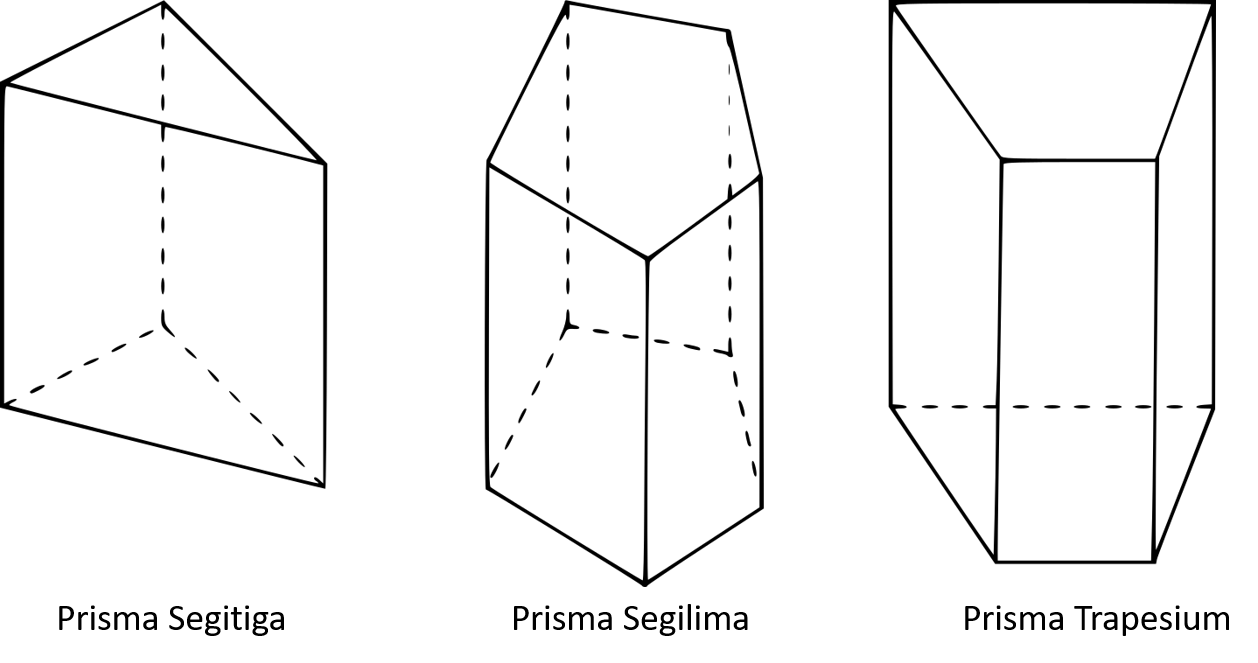
\includegraphics[width=0.6\textwidth]{images/jenisprisma.png}
            \caption{Jenis-jenis Prisma}
            \label{jenisprisma}
        \end{figure}
        \hspace*{1cm}Bangun pada Gambar \ref{jenisprisma} disebut sebagai prisma. Prisma memiliki alas dan tutup yang kongruen (sama bentuk dan ukuran), serta dihubungkan oleh sisi-sisi tegak berbentuk segiempat. Luas permukaan prisma dapat dihitung dengan menjumlahkan luas alas dan tutup, serta luas seluruh sisi tegaknya. Luas permukaan prisma sama dengan luas jaring-jaringnya. Berikut disajikan contoh perhitungan luas permukaan sebuah prisma.
        \begin{enumerate}[label=\arabic*)]
            \item Diketahui sebuah prisma dengan alas berbentuk segitiga siku-siku. Sudut siku-siku terletak di \( \angle ACB \). Jika tinggi prisma adalah 8 cm, maka luas permukaan prisma tersebut adalah \dots\\
            \begin{figure}[H]
                \centering
                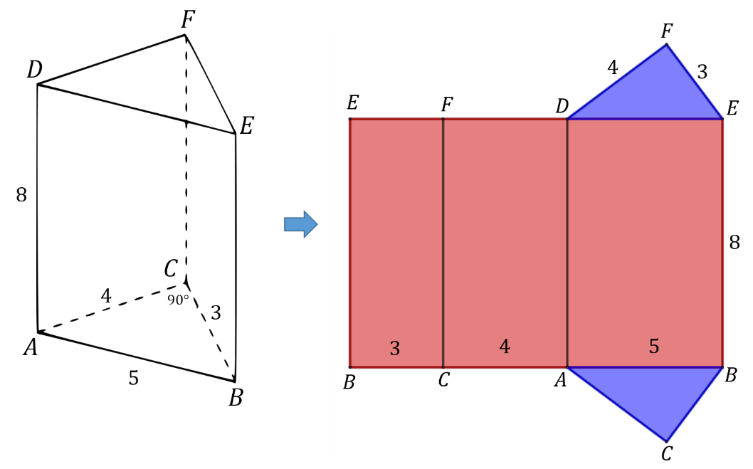
\includegraphics[width=0.6\textwidth]{images/prismasegitigasiku.png}
                \caption{Prisma Segitiga Siku-siku}
                \label{prismasegitigasiku}
            \end{figure}
            Pembahasan:\\
            Luas permukaan prisma dapat dicari dengan terlebih dahulu menentukan luas alas prisma, yang pada Gambar~\ref{prismasegitigasiku} diberi warna biru. Jika alas prisma berbentuk segitiga, maka rumus luas alasnya adalah:\\
            $ L_a = \frac{1}{2} \times a \times t $\\
            $ L_a = \frac{1}{2} \times BC \times AC$\\
            $ L_a = \frac{1}{2} \times 3 \times 4 = 6$\\
            dimana \(a\) adalah panjang alas segitiga, dan \(t\) adalah tinggi segitiga. Untuk selanjutnya bisa dicari luas sisi-sisi tegaknya dengan cara\\
            $ L_t = (BC + CA + AB) \times BE = \text{keliling alas} \times \text{tinggi prisma} $\\
            $ L_t = (3+4+5) \times 8 = 96 $\\
            sehingga didapat luas permukaan prisma\\
            $ L = 2\times L_a + L_t = 2 \times 6 + 96 = 108. $\\
            Jadi luas permukaan prisma tersebut adalah 108 \( \text{cm}^2.\)
        \end{enumerate}
        \hspace*{1cm}Sebelumnya telah dipelajari cara menghitung luas permukaan bangun ruang sisi datar yang memiliki bentuk alas dan tutup yang sama, seperti kubus, balok, dan prisma. Sekarang, bagaimana jika bangun ruang yang akan dicari luas permukaannya memiliki bentuk seperti yang ditunjukkan pada Gambar \ref{jenislimas} berikut?
        \begin{figure}[H]
            \centering
            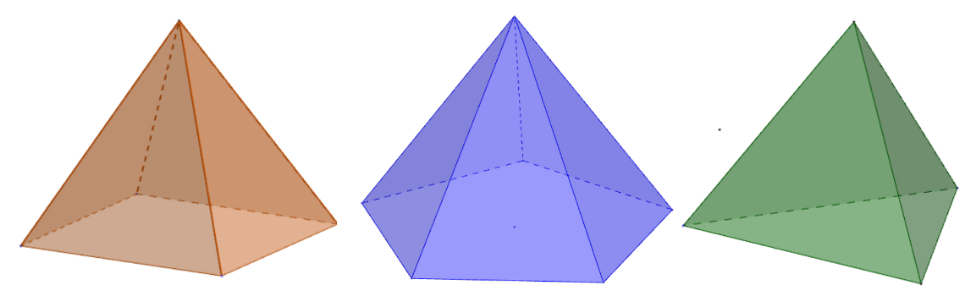
\includegraphics[width=0.6\textwidth]{images/jenislimas.png}
            \caption{Jenis-jenis Limas}
            \label{jenislimas}
        \end{figure}
        \hspace*{1cm}Bangun seperti yang ditunjukkan pada Gambar~\ref{jenislimas} disebut limas. Limas memiliki alas berbentuk bangun datar dan mengerucut ke atas menyerupai piramida. Untuk menghitung luas permukaan limas, terlebih dahulu disajikan jaring-jaring limas segiempat pada Gambar~\ref{limasdanjaring}.
        \begin{figure}[H]
            \centering
            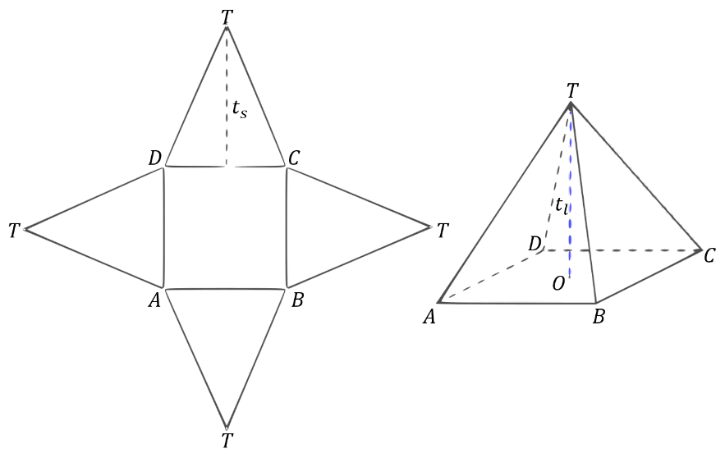
\includegraphics[width=0.6\textwidth]{images/limasdanjaringnya.png}
            \caption{Limas dan Jaring-jaringnya}
            \label{limasdanjaring}
        \end{figure}
        Keterangan:\\
        $ t_s = \text{tinggi sisi tegak} $\\
        $ t_l = \text{tinggi limas} $\\
        $ ABCD = \text{alas limas} $\\
        $ CDT,BCT,ABT,ADT = \text{sisi tegak} $\\
        \hspace*{1cm}Pada limas segiempat seperti yang ditunjukkan pada Gambar~\ref{limasdanjaring}, terdapat empat buah sisi tegak yang memiliki bentuk yang sama, serta satu alas limas yang berbentuk persegi, yaitu alas ABCDABCD. Dengan demikian, luas permukaan limas segiempat dapat dihitung dengan menjumlahkan luas alas dan empat kali luas salah satu sisi tegaknya.
        \begin{equation}
            L_p = 4 \times L_s + L_a
        \end{equation}
        Keterangan:\\
        $ L_p = \text{luas permukaan} $\\
        $ L_s = \text{luas sisi tegak} $\\
        $ L_a = \text{luas alas} $\\
        Diberikan contoh mencari luas permukaan limas seperti berikut.\\
        \begin{enumerate}[label=\arabic*)]
            \item Diketahui limas \( T.ABCD \) dengan alas berbentuk persegi. Jika panjang \( AB = 4\text{ cm} \), dan tinggi sisi tegak limas adalah 5 cm, maka luas permukaan limas tersebut adalah \dots\\
            Pembahasan:\\
            $ L_p = 4 \times L_s + L_a $\\
            $ L_p = 4 \times \frac{1}{2} \times 4 \times 5 + 4 \times 4 $\\
            $ L_p = 40 + 16 = 56 $\\
            Jadi luas permukaan limas tersebut adalah \( 56 \text{ cm}^2 \).\\
        \end{enumerate}

    \end{enumerate}

\end{enumerate}

\textbf{B. Kajian Penelitian yang Relevan}\\
\addcontentsline{toc}{section}{B. Kajian Penelitian yang Relevan}
\hspace*{1cm}Berikut ini adalah beberapa penelitian yang relevan dengan pengembangan media pembelajaran interaktif berbasis Augmented Reality pada materi bangun ruang sisi datar, antara lain:
\begin{enumerate}
    \item Penelitian yang dilakukan oleh \citet{maulana2020} dengan judul \textit{“The Use of Mobile-Based Augmented Reality in Science Learning to Improve Learning Motivation”} bertujuan untuk mengkaji pengaruh penggunaan media berbasis \textit{augmented reality} pada perangkat \textit{Android} terhadap peningkatan motivasi belajar siswa. Penelitian ini menggunakan metode \textit{quasi-experimental} dengan desain \textit{pretest-posttest control group}. Berdasarkan hasil uji statistik menggunakan \textit{SPSS}, diperoleh nilai signifikansi sebesar 0{,}002 yang lebih kecil dari 0{,}025. Hal ini menunjukkan adanya perbedaan skor rata-rata antara kelas kontrol dan kelas eksperimen. Dengan demikian, dapat disimpulkan bahwa pembelajaran menggunakan media \textit{augmented reality} berbasis \textit{Android} berpengaruh positif terhadap proses pembelajaran di kelas, yang ditunjukkan dengan meningkatnya motivasi belajar siswa.
    Persamaan antara penelitian ini dengan penelitian yang sedang dilakukan terletak pada penggunaan media pembelajaran berbasis \textit{augmented reality} pada perangkat \textit{Android}. Adapun perbedaannya terletak pada tujuan penelitian, di mana penelitian ini bertujuan untuk mengembangkan media pembelajaran interaktif berbasis \textit{augmented reality}.
    \item Penelitian yang dilakukan oleh \citet{suprapto2021} dengan judul \textit{“The Use of Physics Pocketbook Based on Augmented Reality on Planetary Motion to Improve Student’s Learning Achievement”}. Penelitian ini bertujuan untuk mengembangkan buku saku berbasis \textit{augmented reality} pada materi gerak planet, fokus pengembangan terletak pada peningkatan prestasi belajar siswa. Penelitian ini menggunakan model \textit{ADDIE} (\textit{Analysis, Design, Development, Implementation,} dan \textit{Evaluation}). Uji coba dilakukan kepada 30 siswa yang terdiri dari 17 perempuan dan 13 laki-laki berusia 16–17 tahun, bertempat di sekolah menengah umum di Surabaya. Parameter evaluasi meliputi kualitas buku saku berbasis \textit{AR}, prestasi belajar siswa, dan luaran penelitian. Teknik analisis data menggunakan statistik deskriptif, \textit{N-gain score}, dan \textit{independent t-test}. Hasil penelitian menunjukkan bahwa: 1) proses pengembangan buku saku berbasis \textit{AR} pada pergerakan planet memenuhi kriteria kualitas produk valid, praktis, dan efektif; 2) prestasi belajar siswa meningkat dilihat dari hasil nilai \textit{pretest-posttest} dengan rata-rata skor \textit{gain} adalah 0{,}63 berkategori sedang, di mana siswa laki-laki berkinerja lebih baik dari siswa perempuan; 3) melalui pengembangan buku saku berbasis \textit{AR}, dihasilkan beberapa artikel di jurnal dan media buku saku berbasis \textit{AR}. Sehingga, rekomendasi dari penelitian ini adalah menggunakan \textit{AR} sebagai media pembelajaran dalam konsep fisika abstrak lainnya. Persamaan dengan penelitian sebelumnya adalah keduanya merupakan penelitian pengembangan media pembelajaran berbasis \textit{augmented reality}. Sedangkan perbedaannya terletak pada materi yang disampaikan, model penelitian, dan bentuk media.
    \item Penelitian yang dilakukan oleh \citet{derlina2020blended} dengan judul \textit{“Blended Learning in English and English-medium Physics Classes Using Augmented Reality, Edmodo, and Tinkercad Media”}. Penelitian ini bertujuan untuk mengetahui efektivitas \textit{blended learning} untuk meningkatkan hasil belajar siswa dalam bahasa Inggris dan fisika dengan menggunakan \textit{AR}, \textit{Edmodo}, dan \textit{TinkerCad}. Ini merupakan penelitian \textit{quasi experiment} dengan data yang diperoleh secara acak dari 70 siswa di SMA 2 Lubuk Pakam, Indonesia. Sampel dibagi menjadi dua kelompok, yang pertama kelas eksperimen yang menerapkan pembelajaran \textit{blended}, dan kedua kelas kontrol yang menerapkan pembelajaran konvensional. Instrumen penelitian berupa tes hasil belajar, berupa tes objektif yang diberikan pada saat \textit{pretest} dan \textit{post-test} dalam bentuk lembar observasi. Efektivitas pembelajaran \textit{blended} dalam meningkatkan hasil belajar siswa dianalisis menggunakan \textit{independent sample t-test} dengan \textit{SPSS 17}. Hasil penelitian menunjukkan bahwa pembelajaran \textit{blended} secara efektif meningkatkan hasil belajar siswa dilihat dari hasil uji \textit{t-test} sampel mandiri dan berpasangan masing-masing sebesar 0{,}148 dan 0{,}000. Dari penelitian ini dapat disimpulkan bahwa pembelajaran \textit{blended} menggunakan \textit{AR}, \textit{Edmodo}, dan \textit{TinkerCad} secara efektif meningkatkan hasil belajar siswa dan membuat siswa menjadi aktif. Perbedaan dengan penelitian sebelumnya adalah, penelitian Derlina dan tim menggunakan tambahan media yaitu \textit{Edmodo} serta dilakukan secara \textit{blended}. Sedangkan persamaannya adalah penggunaan \textit{TinkerCad} untuk membuat objek tiga dimensi.
\end{enumerate}

\textbf{C. Kerangka Berpikir}\\
\addcontentsline{toc}{section}{C. Kerangka Berpikir}
\hspace*{1cm}Kerangka berpikir dalam penelitian dan pengembangan ini dilatarbelakangi oleh permasalahan yang ditemukan di SMP Negeri 3 Kalikajar, yaitu bahan ajar yang digunakan oleh pendidik masih terbatas pada buku teks dan LKS. Selain itu, peserta didik masih mengalami kesulitan dalam menyelesaikan soal-soal yang berkaitan dengan bangun ruang. Berdasarkan permasalahan tersebut, peneliti menawarkan solusi dengan mengembangkan produk berupa media pembelajaran berbasis Augmented Reality. Diharapkan, media pembelajaran berbasis AR ini dapat mempermudah peserta didik dalam memahami materi bangun ruang serta meningkatkan motivasi mereka dalam belajar.\\
\hspace*{1cm}Augmented Reality adalah teknologi yang mampu menampilkan objek 3D seolah-olah terlihat nyata dan menyatu dengan lingkungan sekitar. Teknologi ini sesuai untuk digunakan dalam materi Bangun Ruang Sisi Datar, di mana objek bangun ruang sering kali perlu divisualisasikan secara lebih konkret. Hal ini disebabkan oleh keterbatasan gambar 2D dalam menunjukkan bentuk secara menyeluruh, sehingga dengan Augmented Reality, peserta didik dapat melihat bentuk bangun ruang secara lebih nyata dan mendalam. Proses perancangan media pembelajaran diawali dengan wawancara bersama pendidik mata pelajaran matematika. Dari hasil wawancara diperoleh informasi bahwa peserta didik mengalami kesulitan saat mengerjakan soal yang berkaitan dengan bangun ruang 3D, terutama dalam mengidentifikasi bentuk bangun prisma dan limas.\\
\hspace*{1cm}Proses selanjutnya adalah mempelajari materi bangun ruang dan mengidentifikasi bagian materi yang perlu divisualisasikan ke dalam bentuk Augmented Reality (AR). Setelah materi teridentifikasi, model bangun ruang 3D akan dibuat menggunakan aplikasi Blender. Selanjutnya, materi pembelajaran yang terintegrasi dengan AR dikembangkan dalam bentuk website yang dapat diakses melalui ponsel peserta didik. Media pembelajaran yang telah dikembangkan akan divalidasi oleh ahli, kemudian direvisi sesuai dengan masukan yang diberikan sebelum digunakan dalam proses pembelajaran. Setelah validasi, media akan diuji coba terlebih dahulu pada kelas kecil. Jika masih ditemukan kekurangan, akan dilakukan perbaikan sebelum diujicobakan pada kelas besar. Pada tahap uji coba kelas, peneliti akan mengumpulkan data berupa respons peserta didik terhadap media pembelajaran yang dikembangkan. Alur kerangka berpikir dalam penelitian ini dapat dilihat pada Gambar \ref{diagram} berikut.\\

\begin{center}
\begin{tikzpicture}[
  node distance=1.6cm and 1cm,
  every node/.style={align=center, font=\small},
  scale=0.9, transform shape
]

% Gaya node
\tikzstyle{startstop} = [rectangle, rounded corners, minimum width=3.2cm, minimum height=1cm, text centered, draw=black, fill=white!20]
\tikzstyle{process} = [rectangle, minimum width=3.2cm, minimum height=1cm, text centered, draw=black, fill=white!10]
\tikzstyle{arrow} = [thick,->,>=stealth]

% Jalur utama
\node (start) [startstop] {Identifikasi Masalah:\\
1. Sulit memvisualisasikan objek geometri\\
2. Nilai bangun ruang di bawah KKM\\
3. Menggambar 3D masih di papan tulis};

\node (desain) [process, below=of start] {Desain Produk};
\node (kembangkan) [process, below=of desain] {Mengembangkan Media Pembelajaran\\Berbasis AR};
\node (validasi) [process, below=of kembangkan] {Melakukan Validasi};

% Paralel validasi
\node (validasi_media) [process, left=3cm of validasi] {Validasi Ahli Media};
\node (validasi_materi) [process, right=3cm of validasi] {Validasi Ahli Materi};

\node (revisi_media) [process, below=of validasi_media] {Revisi Media};
\node (revisi_materi) [process, below=of validasi_materi] {Revisi Materi};

% Titik koordinat di bawah revisi
\node (bawah_media) [below=0.4cm of revisi_media] {};
\node (bawah_materi) [below=0.4cm of revisi_materi] {};

% Titik gabung di bawah tengah
\node (merge) [coordinate] at ($(bawah_media)!0.5!(bawah_materi)$) {};

% Lanjut ke bawah
\node (uji_coba) [process, below=1.6cm of merge] {Melakukan Uji Coba};
\node (revisi2) [process, below=of uji_coba] {Revisi Setelah Uji Coba};
\node (produk_akhir) [startstop, below=of revisi2] {Produk Akhir};

% Panah utama
\draw [arrow] (start) -- (desain);
\draw [arrow] (desain) -- (kembangkan);
\draw [arrow] (kembangkan) -- (validasi);

% Panah validasi
\draw [arrow] (validasi) -- (validasi_media);
\draw [arrow] (validasi) -- (validasi_materi);
\draw [arrow] (validasi_media) -- (revisi_media);
\draw [arrow] (validasi_materi) -- (revisi_materi);

% Dari revisi ke titik merge (lurus)
\draw [arrow] (revisi_media.south) -- (bawah_media.center);
\draw [arrow] (revisi_materi.south) -- (bawah_materi.center);
\draw [arrow] (bawah_media.center) -- (merge);
\draw [arrow] (bawah_materi.center) -- (merge);

% Lanjut ke bawah
\draw [arrow] (merge) -- (uji_coba);
\draw [arrow] (uji_coba) -- (revisi2);
\draw [arrow] (revisi2) -- (produk_akhir);

\end{tikzpicture}
\end{center}
\begin{figure}[H]
    \caption{Alur Kerangka Berpikir}
    \label{diagram}
\end{figure}